\documentclass[20]{article}
\usepackage{amsmath,amssymb,amsthm}
\usepackage{mathtools}
\usepackage[legalpaper, portrait, margin=1in]{geometry}
\usepackage{TikZ}
\usepackage{amsfonts}
\usepackage[mathscr]{eucal}
%\eta
\begin{document}

	\pagenumbering{gobble} %Remove the page counter
	\noindent 1164 \hfill Found Comput Math (2018) 18:1131--1198\\
	\rule{\textwidth}{0.4pt}\\
	\indent 
	\large
	\\
	%
	$\indent\Bigg|\Bigg|
	\dfrac{1}{m}\sum\limits_{k=1}^{m}|a_k(1)|^2
	\begin{bmatrix}
		|a_k(1)|^2 & a_k(1)\tilde{\textbf{\textit{a}}}_k^*\\
		\overline{a_k(1)}\tilde{\textbf{\textit{a}}}_k & \tilde{\textbf{\textit{a}}}_k\tilde{\textbf{\textit{a}}}_k^*
	\end{bmatrix} - (\textbf{\textit{e}}_l\textbf{\textit{e}}_l^* + \textbf{\textit{I}})
	\Bigg|\Bigg|$\\
	% Next equation
	%
	$\indent\indent\leq\Bigg|
	\dfrac{1}{m}\sum\limits_{k=1}^{m}(|a_k(1)|^4-2)
	\Bigg|+\Bigg|\Bigg|
	\dfrac{1}{m}\sum\limits_{k=1}^{m}|a_k(1)|^2
	\begin{bmatrix}
		0 & a_k(1)\tilde{\textbf{\textit{a}}}_k^*\\
		a_k(1)\tilde{\textbf{\textit{a}}}_k & \textbf{0}
	\end{bmatrix}\Bigg|\Bigg|$\\
	% Next Equation
	%
	$\indent\indent\indent
	+\Bigg|\Bigg|
	\dfrac{1}{m}\sum\limits_{k=1}^{m}|a_k(1)|^2
	(\tilde{\textbf{\textit{a}}}_i\tilde{\textbf{\textit{a}}}_k^* - \textbf{\textit{I}}_{n-1})
	\Bigg|\Bigg|+\Bigg|
	\dfrac{1}{m}\sum\limits_{k=1}^{m}(|a_k(1)|^2-1)
	\Bigg|.$\\\\
	%
	By Chebyshev's inequality, we have with probability at least 1 - $c_1\delta^{-2}m^{-1}$, \\\\
	%
	$\indent\indent\Bigg|
	\dfrac{1}{m}\sum\limits_{k=1}^{m}(|a_k(1)|^4-2)| 
	\leq \dfrac{\delta}{4} 
	and 
	\Bigg|
	\dfrac{1}{m}\sum\limits_{k=1}^{m}(|a_k(1)|^2-1)
	\Bigg| 
	\leq \dfrac{\delta}{4}$.\\\\
	%
	To bound the second term, we note that\\
	%
	\begin{align*}
		\indent\Bigg|\Bigg|
		\dfrac{1}{m}\sum\limits_{k=1}^{m}|a_k(1)|^2
		\begin{bmatrix}
			0 & a_k(1)\tilde{\textbf{\textit{a}}}_k^*\\
			\overline{a_k(1)}\tilde{\textbf{\textit{a}}}_k & \textbf{0}
		\end{bmatrix}
		\Bigg|\Bigg| &= \Bigg|\Bigg|
		\dfrac{1}{m}\sum\limits_{k=1}^{m}|a_k(1)|^2a_k(1)\tilde{\textbf{\textit{a}}}_k^*
		\Bigg|\Bigg|\\
		&= \underset{\textbf{\textit{w}}\in\mathbb{C}^{n-1}:||\textbf{\textit{w}}||=1}{\textnormal{sup}} \dfrac{1}{m}\sum\limits_{k=1}^{m}|a_k(1)|^2a_k(1)\tilde{\textbf{\textit{a}}}_k^*\textbf{\textit{w}}.
	\end{align*}\\
	%
	For all $\textbf{\textit{w}}$ and all $\textit{k}$ $\in$ [$\textit{m}$], $\tilde{\textbf{\textit{a}}}_k^*\textbf{\textit{w}}$ is distributed as $\mathcal{C}\mathcal{N}$(1) that is independent of the \{$a_k$(1)\} sequence. So for one realization of \{$a_k$(1)\}, the Hoeffding-type inequality of Lemma 29 implies\\\\
	%
	$\indent\indent
	\mathbb{P}\Bigg[
		\dfrac{1}{m}\sum\limits_{k=1}^{m}|a_k(1)|^2a_k(1)\tilde{\textbf{\textit{a}}}_k^*\textbf{\textit{w}} > t
	\Bigg]
	\leq
	\textnormal{e} \hspace{3pt} \textnormal{exp}
	\Bigg( 
		-\dfrac{c_2m^2t^2}{\sum_{k=1}^m|a_k(1)|^6}
	\Bigg).$\\\\
	%
	for any $\textit{\textbf{w}}$ with $||\textit{\textbf{w}}||$ = 1 and any $t > 0$. Taking $t$ = $\delta$/8, together with a union bound on a 1/2-net on the sphere, we obtain\\\\
	%
	$\mathbb{P}
	\Bigg[
		\Bigg|\Bigg|
			\dfrac{1}{m}\sum\limits_{k=1}^{m}|a_k(1)|^2a_k(1)\tilde{\textbf{\textit{a}}}_k^*
		\Bigg|\Bigg|
		 > \delta/4
	\Bigg]
	\leq \textnormal{e} \hspace{3pt} \textnormal{exp}
	\Bigg(
		-\dfrac{c_2m^2t^2}{64\sum_{k=1}^m|a_k(1)|^6}+12(n-1)
	\Bigg).
	$\\\\
	%
	Now an application of Chebyshev's inequality give that $\sum_{k=1}^m|a_k(1)|^6 \leq$ 20m with probability at least 1 - $c_3$m$^{-1}$. Substituting this into the above, we concluded that whenever $m \geq C_4\delta^{-2}n$ for some sufficiently large $C_4$,\\\\
	%
	$\indent\indent\indent\indent
	\Bigg|\Bigg|
		\dfrac{1}{m}\sum\limits_{k=1}^{m}|a_k(1)|^2a_k(1)\tilde{\textbf{\textit{a}}}_k^*
	\Bigg|\Bigg|
	\leq
	\delta/4$\\\\
	%
	with probability at least 1 - $c_3m$ - exp (-$c_5\delta^2\textit{m}$).
	%
	\newpage
	\pagenumbering{gobble} 
	\noindent 1268 \hfill Found Comput Math (2018) 18:1245--1297\\
	\rule{\textwidth}{0.4pt}\\
	%
	\indent The previous results are required to show that the interleavings are in a sense closed under composition, e.g., composing two left interleavings (with a suitable ordering of terms), yields a left interleaving (with an additive approximation factor). Now, we show the more interesting property: Most combinations of the different notions of interleavings do not interact, i.e., composition yields the maximum of the two rather than an additive factor. First, we show that if compositions is \textbf{not} in the natural order as in Propositions 4.11 and 4.10, the interleavings do not yield an additive factor.\\\\
	%
	\textbf{Propositions 4.12} \textit{Suppose one of the following two possible holds,}\\\\
	%
	$\indent\indent
	M \overset{2\epsilon}{\tilde{}}_L N\indent
	and\indent
	P \overset{2\epsilon}{\tilde{}}_L N,\indent
	or\indent
	M \overset{2\epsilon}{\tilde{}}_R N\indent
	and\indent
	P \overset{2\epsilon}{\tilde{}}_R N,\indent$\\\\
	%
	\textit{then} $M \overset{2\epsilon}{\tilde{}}P$.\\\\
	%
	\textit{Proof} In the first case, we have the following two exact sequences:\\\\
	%
	$\indent\indent
	0 \rightarrow M \overset{i}{\rightarrow} N \overset{f}{\rightarrow} X \rightarrow 0
	\indent
	\textnormal{and}
	\indent
	0 \rightarrow P \overset{g}{\rightarrow} N \overset{j}{\rightarrow} Y \rightarrow 0$\\\\
	%
	Similarly in the second case, we have:\\\\
	%
	$\indent\indent
	0 \rightarrow X \overset{f}{\rightarrow} M \overset{i}{\rightarrow} N \rightarrow 0
	\indent
	\textnormal{and}
	\indent
	0 \rightarrow Y \overset{j}{\rightarrow} P \overset{g}{\rightarrow} N \rightarrow 0$\\\\
	%
	In both cases, by assumption $X \overset{\epsilon}{\tilde{}} 0$ and $Y \overset{\epsilon}{\tilde{}} 0$. By propositions 4.1 and 4.2, for both cases there are 2$\epsilon$-interleavings ($\phi,\psi$) of \textit{M} and \textit{N} and ($\eta,\theta$) of \textit{P} and \textit{N}. These fit into the following commutative diagram, where the horizontal arrows are ordinary morphisms and all other arrows are 2$\epsilon$-morphisms.\\\\
	%
	$\indent\indent\indent\indent\indent\indent
	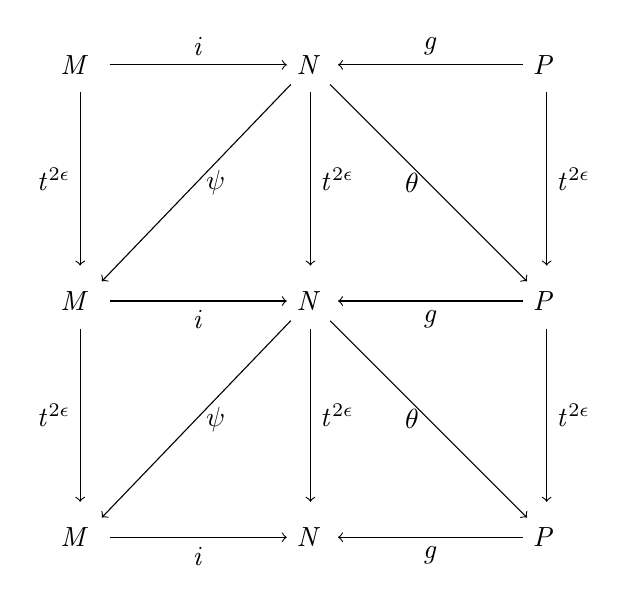
\begin{tikzpicture}
		\filldraw[black] (0,0) circle (0pt) node[anchor=west]{\textit{M}};
		\draw[black,->](0.75,0) -- node[anchor=north]{\textit{i}} (3,0);
		\filldraw[black] (3,0) circle (0pt) node[anchor=west]{\textit{N}};
		\draw[black,<-](3.65,0) -- node[anchor=north]{\textit{g}} (6,0);
		\filldraw[black] (6,0) circle (0pt) node[anchor=west]{\textit{P}};
		%
		\filldraw[black] (0,3) circle (0pt) node[anchor=west]{\textit{M}};
		\draw[black,->](0.75,3) -- node[anchor=north]{\textit{i}} (3,3);
		\filldraw[black] (3,3) circle (0pt) node[anchor=west]{\textit{N}};
		\draw[black,<-](3.65,3) -- node[anchor=north]{\textit{g}} (6,3);
		\filldraw[black] (6,3) circle (0pt) node[anchor=west]{\textit{P}};
		%
		\filldraw[black] (0,6) circle (0pt) node[anchor=west]{\textit{M}};
		\draw[black,->](0.75,6) -- node[anchor=south]{\textit{i}} (3,6);
		\filldraw[black] (3,6) circle (0pt) node[anchor=west]{\textit{N}};
		\draw[black,<-](3.65,6) -- node[anchor=south]{\textit{g}} (6,6);
		\filldraw[black] (6,6) circle (0pt) node[anchor=west]{\textit{P}};
		%
		\draw[black,->](.375,5.65) -- node[anchor=east]{\textit{t}$^{2\epsilon}$} (.375,3.45);
		\draw[black,->](3.3,5.65) -- node[anchor=west]{\textit{t}$^{2\epsilon}$} (3.3,3.45);
		\draw[black,->](6.3,5.65) -- node[anchor=west]{\textit{t}$^{2\epsilon}$} (6.3,3.45);
		%
		\draw[black,->](.375,2.65) -- node[anchor=east]{\textit{t}$^{2\epsilon}$} (.375,.45);
		\draw[black,->](3.3,2.65) -- node[anchor=west]{\textit{t}$^{2\epsilon}$} (3.3,.45);
		\draw[black,->](6.3,2.65) -- node[anchor=west]{\textit{t}$^{2\epsilon}$} (6.3,.45);
		%
		\draw[black,->](3.05,5.75) -- node[anchor=west]{$\psi$} (.65,3.25);
		\draw[black,->](3.05,2.75) -- node[anchor=west]{$\psi$} (.65,.25);
		%
		\draw[black,->](3.55,5.75) -- node[anchor=east]{$\theta$} (6.05,3.25);
		\draw[black,->](3.55,2.75) -- node[anchor=east]{$\theta$} (6.05,.25);
		%\psi\theta\qed
	\end{tikzpicture}$\\\\
	%
	By inspection of this diagram, we see that ($\theta$\textit{i},$\psi$\textit{g}) is a 2$\epsilon$-interleaving of \textit{M} and $\textit{P}_{\qed}$.\\\\
	%
	\textbf{Propositions 4.13} \textit{Suppose one of the following two possibilities holds,}\\\\
	%
	$\indent\indent
	N \overset{2\epsilon}{\tilde{}}_L M
	\indent
	and
	\indent
	N \overset{2\epsilon}{\tilde{}}_L P,
	\indent
	or
	\indent
	N \overset{2\epsilon}{\tilde{}}_R M
	\indent
	and
	\indent
	N \overset{2\epsilon}{\tilde{}}_R P,$
	

\end{document}